% https://ask.latexstudio.net/ask/question/17817.html
\documentclass[tikz,border=1cm]{standalone}
\usepackage{physics2}
\usephysicsmodule{ab.braket}
\begin{document}
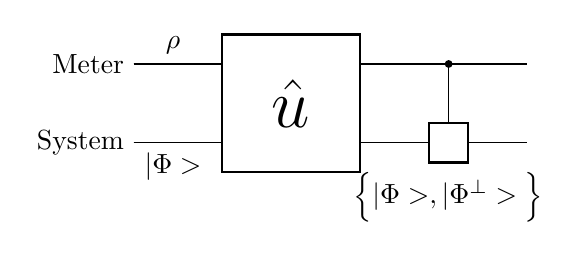
\begin{tikzpicture}
  \draw (0,.5) 
    node[rectangle,anchor=east] {Meter} 
    edge node[above] {$\rho$} 
    ++(1,0) -- ++(5,0);%
  \draw (0,-.5) 
    node[rectangle,anchor=east] {System} 
    edge node[below] {$\ket|\Phi>$} 
    ++(1,0) -- ++(5,0);%
  \node[draw,thick,fill=white,rectangle,minimum size=1.75cm,font=\Huge] at (2,0) {$\hat{u}$};
  \draw (4,.5) 
    node[circle,fill,inner sep=1pt] {} -- (4,-.5) 
    node[draw,thick,fill=white,rectangle,minimum size=.5cm] {} 
    node[below=.25cm] {$\Big\{\ket|\Phi>,\ket|\Phi^\perp>\Big\}$};
\end{tikzpicture}
\end{document}